\chapter{Subfigures}

So far we have been using the |caption| package to add captions to multiple figures, that are numbered individually, but how about if you want to have only one caption and number the subfigures alphabetically. If you want to have |subfigures| with distinct caption, you use the |subfig| package \citep{subfigure}. A newer package \ctan{subcaption} is also now available with the |caption| suite and we will discuss this also. The two packages are incompatible and the recommendation is to use the |subcaption| package. In the |phd| class we load the |caption| package which also loads the |subcaption| package. The latter is to be preferred as it integrates better both with captions as well as the |hyperref| package.

\begin{figure}[h]
\centering
\begin{minipage}[b]{.3\linewidth}
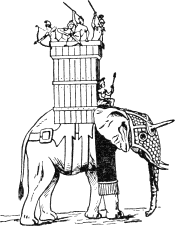
\includegraphics[width=4cm]{./graphics/pic37.png}\hspace{1em}
\subcaption{First fighting elephant}\label{fig:1a}
\end{minipage}\hspace{1em}
\begin{minipage}[b]{.3\linewidth}
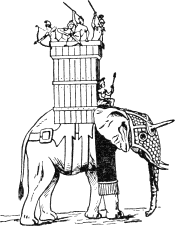
\includegraphics[width=4cm]{./graphics/pic37.png}\hspace{1em}
\subcaption{Second fighting  elephant}\label{fig:1b}
\end{minipage}\hspace{1em}
\begin{minipage}[b]{.3\linewidth}
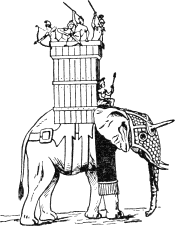
\includegraphics[width=4cm]{./graphics/pic37.png}\hspace{1em}
\subcaption{Third fighting elephant}\label{fig:1c}
\end{minipage}
\caption{Three fighting elephants example}
\end{figure}

You can put as many figures as you like on a page, but a word of warning, you may need to make some manual adjustments before you get it right. The package provides support for the manipulation and reference of small or \enquote{sub} floats within a single floating (e.g., figure or table) environment It is convenient to use this
package when your sub-floats are to be separately captioned, referenced, or when such
sub-captions are to be included on a List of Floats page.

The package is a replacement for the |subfigure| package, from which it was derived.
However, the new |subfig| package is not completely backward compatible.
Therefore, a new name was called for. The newer package is smaller and easier to use
than the older package, however, it now uses the following additional packages,  |caption| (required),  |everysel| (optional),
keyval (required),  |ragged2e| (optional). All these packages are included with the |phd| auto package manager.

It will work without the |ragged2e| and |everysel| packages if you do not use the following
justification options: \enquote{Center}, \enquote{RaggedRight} and \enquote{RaggedLeft}. The other justification
options \enquote{center}, \enquote{raggedright} and \enquote{raggedleft} will work without the above two packages. If the ragged2e package is present, than the caption package will load it and it
will, in turn, load the everysel package. This happens whether or not you will be using
the justification options that require it. If it cannot find the ragged2e package, than the
caption package will print a message that \enquote{RaggedRight}, etc. will not be available.

\section{Subcaption environments}

The |subcaption| package offers an environment for subfigures, which are essentially minipages. Within the environment, the normal caption command can be used rather than the \cmd{\subcaption}.

\begin{figure}%
    \centering
    \captionsetup[figure]{margin=3pt}%
    \begin{subfigure}[b]{.35\linewidth}
    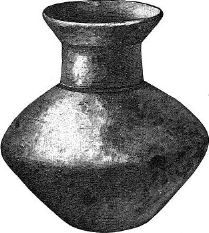
\includegraphics[scale=0.65]{./graphics/fig155.jpg} 
    \label{fig:one}
    \caption{First Caption}
    \end{subfigure}\hspace{2em}
    \begin{subfigure}[b]{.35\linewidth}
    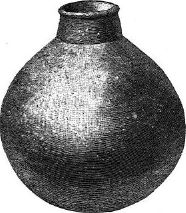
\includegraphics[scale=0.65]{./graphics/fig156.jpg} 
    \caption{First Caption}
    \end{subfigure}
    \caption{Two subfigures side by side.}
    \label{fig:two}
\end{figure}

The sub-figures can be referenced the same way as normal referencing.

\begin{quote}
 A low bottle-shaped vase, of yellowish ware, with flaring rim and somewhat flattened body. Height, 5 inches; width 5 inches. \ref{fig:one}


A well-made bottle shaped vase, with low neck and globular body, somewhat conical above. Color dark brownish. $7\frac{1}{2}$ inches in height. Shown in Figure~\ref{fig:two}.
\end{quote}

\begin{figure}[htp]
  \centering
  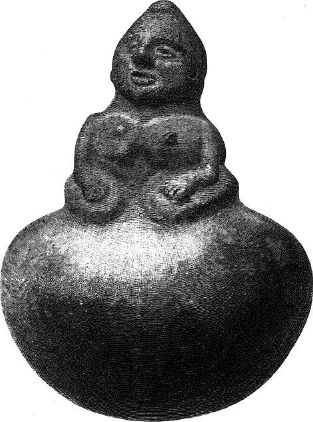
\includegraphics[width=0.5\linewidth]{./graphics/fig175.jpg}
  \vspace{3\baselineskip}

   \centerline{\textsc{From the tomb of a Pull\= arius.}}
  \label{fig:marginfig1}
  \caption{ effigy vase of the dark ware. The body is globular. A kneeling human figure forms the neck. The mouth of the vessel occurs at the back of the head—a rule in this class of vessels. Is is finely made and symmetrical. 9.75 inches high and 7 inches in diameter. being larger than the above two it is preferable to scale it to give the reader an indication.}
\end{figure}

The above figure is an Based on the figure width, you may also need to adjust the distance between the figures to ensure that the whitespace is just about right. For screen reading this can be increased and for printed works you may wish to make it less.

\begin{teXXX}
\begin{figure}[htb]
\begin{subfigure}[b]{.5\linewidth}
\centering\large A
\captionsetup{skip=3pt}
\caption{A subfigure}\label{fig:1a}
\end{subfigure}
\end{figure}
\end{teXXX}

\begin{comment}
\begin{figure}[htp]%
    \captionsetup[figure]{margin=3pt}%
    \subfloat[One subone.\label{fig:one}]
     {{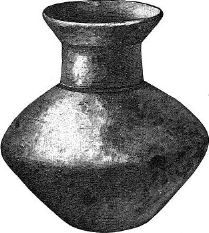
\includegraphics[scale=0.65]{./graphics/fig155.jpg}}}
    \hspace{1cm}
    \subfloat[One subtwo.\label{fig:two} --- but this one has a
     very very long caption.  So long that it continues over into
     other lines so that we can test the list-of line settings.]%
      {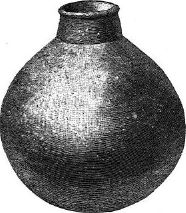
\includegraphics[scale=0.65]{./graphics/fig156.jpg}}
     \\[-10pt]
    \caption{First figure --- but this one has a very very long caption.
     So long that it continues over into a second line so that we can
     test the margin setting and centering of the caption command in the
     full page mode.}%
    \label{fig:Afirst}%
    \caption{Typical pottery from Oklahoma (\emph{Smithsonian}).}%
    \label{fig:Athird}%
\end{figure}
\end{comment}

The figures have been placed using the code below:

\begin{verbatim}
\begin{figure}%
    \captionsetup[figure]{margin=3pt}%
    \subfloat[One subone.\label{fig:one}]
     {{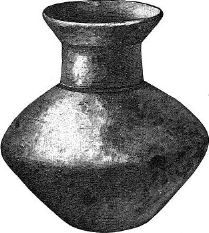
\includegraphics[scale=0.65]{./graphics/fig155.jpg}}}
    \hspace{1cm}
    \subfloat[One subtwo.\label{fig:two} --- but this one has a
     very very long caption.  So long that it continues over into
     other lines so that we can test the list-of line settings.]%
      {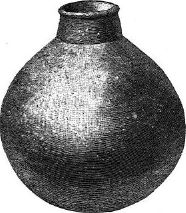
\includegraphics[scale=0.65]{./graphics/fig156.jpg}}
     \\[-10pt]
 \caption{First figure but this one has a very very long caption.
 So long that it continues over into a second line so that we can
 test the margin setting and centering of the caption command in the
 full page mode.}%
 \label{fig:Afirst}%
 \caption{Typical pottery from Oklahoma (\emph{Smithsonian}).}%
 \label{fig:Athird}%
\end{figure}
\end{verbatim}

As you can observe, the |subcaption| package treats the two figures as one and places them side by side. Its trickery is to get them to line up, nicely and to provide all the necessary parameters for the captions. It is a feature-rich package and we will spent some time to explore it. The command |subfloat|, is used to denote the |subfigure|. The rest are self-explanatory. Note that the use of |\hspace{1cm}| to make these two figures come closer together. In the previous listings, |\hfill| was used to space them out as wide as possible. The command |captionsetup| is used to let the package know that we are captioning figures and not tables. (In this book all captions are placed in the side-margins, where God meant them to be! If you use the same code in another package they will be placed underneath the figures.



